% 来源：OEBPS/Text/Section0001_split_004.xhtml#sigil_toc_id_34

\BookChapter{23}
\section[第23章\q 比赛就是为了赢：风险/成长水桶]{第23章\\ 比赛就是为了赢：风险/成长水桶}

\begin{BookQuote}
赢家并不是那个开着最快赛车的人。赢家是那个拒绝输掉比赛的人。

\hfill ——老戴尔·伊恩哈德
\end{BookQuote}

风险/成长水桶是每个人都要去的地方。为什么？因为它很吸引人，它让人很兴奋，很激动！这又是为什么？原因非常简单，一个字“钱”！你能在这里得到高得多的收益率，但是其中的关键字是“能”。能赚钱也能亏钱。你也能输掉你储蓄和投资的所有财富。所以不管你放进你的风险/成长水桶的是什么样的投资，你必须做好心理准备，你可能会亏掉一部分本金，甚至亏得精光，因为你的安全保障措施事先没有做到位。我们怎么知道这一点？因为生命中的任何一件事情，包括市场在内，都像海浪一样，一波接着一波，一个循环接着一个循环，既有上涨的时候，也有下跌的时候。一个人投资某一类资产，碰巧它涨得非常好——不管是房地产、股票、债券、商品或者其他资产——要是他觉得这种涨势将会永远继续下去，他觉得“这次跟以前不一样”，那你就等着看吧，市场早晚会给他当头一棒，让他幡然悔悟，这次仍然和以前一样，有涨必有跌。我为了写本书，采访了约翰·博格，他一再重复那句魔咒：“市场总会回归到平均水平。”（他的意思是，有涨必有跌，有跌必有涨。）瑞·达利欧的一句话一定吸引了你的注意，他说：“不管你最喜欢的投资是什么，你等着看好了，你这辈子肯定会遇到这类资产下跌50\%\textasciitilde{}70\%的情况。”尽管风险/成长水桶的上涨潜力没有上限，但是你绝对不要忘了，你也有可能全部亏光（或者至少会亏掉相当大的一部分）。这正是为什么我称之为风险/成长水桶，而不是成长/风险水桶。成长不能保证，但是风险肯定会有。

那么你应该把哪些投资放在风险/成长水桶里？

下面我列出了7类投资，可以供你参考。

1.股权

股权其实就是股票的另外一种叫法，相当于学名，它可以是你持有私人企业的一部分所有权，也可以是你用金融投资工具同时持有很多企业的所有权，比如你买了公募基金、指数基金或者ETF（交易所交易基金）。这等于你同时持有几百只股票，同时身为这几家上市公司的股东。

ETF可以说是股票市场最具人气的明星，它增长迅速，2011—2014年，ETF规模增长了20倍，持股市值超过2万亿美元。但是ETF究竟是什么？其实ETF和公募基金或指数基金本质上是一样的，分散投资很多股票或其他种类资产，由此形成一个资产包，但是它和开放式基金或指数基金不同的是，你可以在股市上买卖ETF，就像买卖个股一样。而大多数ETF都是追踪一个主题（小盘股、股票、市政债券、黄金，或者追踪一个指数）的，但是你要是投资一个指数基金或者开放式基金，必须等到交易日结束后你才能买入或者卖出，而ETF在一整天的交易时间内可以像股票一样随时交易。专家说，如果你喜欢指数基金这种投资思路，但是你又想择时交易，在交易时段内看到价格低了，就低位买入，看到价格高了，就趁机高位卖出，那么ETF会很适合你。但是这是交易，而不是投资。你试图选择市场时机，频繁交易，这样做会给你自己带来非常高的风险。

还有另外一个不同：你买了一份ETF，其实你买的不是真正的股票、债券、商品，或者其他包括在这个基金里的东西，你其实买入了一份投资基金，由这只基金来持有这些资产。发行ETF的基金公司承诺，你买ETF的投资收益和你自己直接持有这些资产是一样的。这听起来很复杂，其实没什么难的。

很多人喜欢ETF，是因为ETF能给你带来范围非常宽广的分散投资，和你自己操作这样的分散投资相比，成本低得多。事实上，很多ETF的费用要比传统指数基金更低，有时所需的最小投资金额也更低。而且因为ETF追踪的是指数，建仓之后，持股稳定不变，只有指数调整少量成分股时，才会引起ETF跟着调整持仓，所以一年下来，很少交易，自然不会有很多产生资本利得的收益，因此ETF有很高的税收效率。（不过，也有一种更加趋向于主动管理型的ETF在市场上出现，这降低了它的税收效率。）

你应该投资ETF吗？约翰·博格——先锋公司的创始人（先锋公司同样也提供很多种类的ETF）——告诉我，他觉得持有投资范围很广、分散的指数型ETF，当然一点儿错没有。但是他警告，有些种类的ETF对于个人投资者来说太专业了，最好别碰。“你用ETF，不但能赌市场，还可以赌国家，赌行业板块，你可能是对的，也可能是错的。”

2.高收益债

你也许知道，高收益债其实就是垃圾债券，称它们为垃圾是有理由的。这些债券只有最低的安全评级，你可以得到高收益率的息票（高于更加安全的债券的收益率），但是这只是因为你冒了大风险。对于一个新手来说，你最好别碰它们，回过头去读一读前面的债券概述，就在上一章的末尾。

3.房地产

我们都知道，房地产能产生巨大的收益，你可能对房地产这个种类已经知道得很多了。但是你可能不知道，除了买房卖房这个传统方式之外，还有很多方式可以投资不动产。你可以投资一套住宅，把它租出去，得到租金收入。你可以买不动产，重新装修，然后短期内转手卖出。你可以投资第一信托契约。你可以买商铺（商业不动产）或者一套公寓。我前面讲过，我最喜欢的房地产投资种类之一，就是投资养老住宅，你既可以得到稳定的租金收入或分红收入，又可以得到未来资产升值的收益。你可以买房地产投资信托基金。这种基金持有大量的商业不动产（或者抵押贷款），然后再向小投资者出售基金份额，就像开放式基金一样。房地产投资信托基金可以像股票一样交易，你可以买入一只房地产投资信托基金指数基金，这可以让你分散投资到很多不同的房地产投资信托基金上。

为了投资增值，诺贝尔经济学奖获得者罗伯特·席勒告诉我，你最好投资房地产投资信托基金，而不是投资自住型的房产（它属于安全/安心水桶）。购买商业地产或者公寓，对于我来说是一个更好的投资，它胜过自己买套房子，因为前者要租出去更加容易。当然这可能是会变的。和任何一项投资一样，你必须停下来，好好想想自己赌的是什么。你赌的是房地产的价格会随着时间的推移而上涨，但是这没有保障，所以要放在风险/成长水桶里。如果房地产价格确实上涨了，你就会有很好的收益率，如果它没有上涨，你什么也得不到，甚至会输得精光。当你自己买房子的时候，你赌的是你的房子价格会上涨。当你购买与之关联的房地产类产品（出租单位、公寓楼、商业地产、房地产投资信托基金或持有相关指数基金）时，席勒指出，你有两种赢的方式：一方面你可以持续获得收入，另一方面如果这些房地产升值，你就有机会赚钱了，你可以在升值之后把它们高价卖出。

4.商品期货

这个种类的资产包括：黄金、白银、原油、咖啡。很多年来，大多数人认为黄金是最安全的投资天堂，它在他们的安全/安心水桶里占了一大部分。传统的智慧认为，乱世藏黄金，在不确定的动荡年代，黄金的价值只会涨。结果，黄金的价格在2013年跌幅超过25\%！人们这才明白，黄金也会暴跌。为什么你要投资黄金？你可以持有一小部分黄金，你可以这样说：“这是为了避免纸币消失，这能给我带来一份小小的安全感。”你知道，如果整个世界都崩溃了，政府也崩溃了，僵尸入侵，统治整个世界，至少你还有点儿黄金或者白银让你能买上一条小船，航行在大海上。（忽然一想，僵尸也会游泳啊！）另外，黄金也可能属于你的风险/成长水桶。你投资黄金是为了保护自己，对抗通货膨胀，或者作为平衡投资组合的一个组成部分，我们后面会学到如何在投资组合中配置一部分黄金。但是你必须接受风险。不要愚弄自己，你买黄金，其实你是在赌金价会上涨。和其他很多投资不同，黄金这种投资是绝对不会产生收入的，而你投资股票会有分红收入，投资房地产会有租金收入，投资债券会有利息收入，而投资黄金什么收入也没有。所以不管投资黄金值不值得，风险是肯定存在的，所以黄金肯定应该属于风险/成长水桶。这并不是指责、攻击黄金，事实上在合适的经济情况下，黄金可能成为超级投资明星。正是因为这个原因，你将会看到，在你的投资组合中持有一小部分黄金，会非常有用。

5.外汇

想炒日元吗？其实所有的外汇，就是外国的纸币，也只是一张纸而已。外汇投资，其实纯粹是投机。有人炒外汇发了大财，但更多的人亏了大钱。那些内心不够强大的人不适合炒外汇。

6.收藏

艺术品、葡萄酒、钱币、汽车、古董，还有很多其他东西，都可以收藏。同样，了解值得收藏的资产，你要有非常专业的知识，还要有很多时间。

7.结构化票据

前面我们说过了，结构化票据属于安全/安心水桶。同一个东西怎么能够同时属于两个水桶？因为市场上有各种类型的结构化票据，有些百分之百保本，可以进入你的安全/安心水桶——发行票据的银行只要在财务上非常稳健，就肯定能够保本。另外，还有其他种类的票据，可以给你带来更高的潜在收益，但是如果票据挂钩的指数下跌，你的本金只能部分保本。比如你买了一个票据，有25\%保本，这意味着只要股市下跌幅度最高不超过25\%，你就一分钱也不会损失。如果股市继续下跌，跌了35\%，超过25\%的保本范围，你就得不到保护了，就要亏本10\%。但是因为你承担的风险更大，你得到的上行收益相应也更多——有时会高达挂钩指数上行收益的150\%。比如，如果股市上涨了10\%，你就可以得到15\%的收益。所以，你将来得到更大的收益是可能的，但是你承担了更大的风险，这是一定的。再一次提醒你，结构化票据应该用你的个人退休金账户购买，它能让你脱离所有过度征收的费用，然后给你带来更高的税后收益。

\begin{BookQuote}
安全并不是意外发生的。

\hfill ——佛罗里达州高速公路上的标语
\end{BookQuote}

到现在为止，我们已经讲了一些投资工具/资产，它们可以纳入你的风险/成长水桶，让这个水桶里的投资更加分散。你可能疑惑不解，为什么我没有把一些风险更大的投资工具包括在内？这些投资工具现在还蛮流行的：看涨和看跌期权、信用违约债券，还有一大堆稀奇古怪、深奥难懂的金融工具，现在交易者在市场上都能买到。你如果是富豪，也许会聘请专业受托人投资顾问，帮你仔细看一看如何使用这些投资工具。但是你务必清醒地认识到：只要一玩这种游戏，你就再也不是一个纯粹的投资者了，你变成了一个投机者。这就是所谓的动量交易。你必须认识到，如果你玩这种游戏出错了，你会把本金亏得精光。这还不止，你还要欠上一屁股债，从此天天被人追债。因为本书讲的通向财务自由之路的途径是多存钱，多投资，用复利实现增长，所以在此讨论这类动量交易的资产并不合适。

\subsection{现在进入游戏的时候到了}

好了，现在你了解哪些资产选手属于你的资产配置水桶团队了，现在你也知道打造一个赢家团队的关键所在：分散，分散，还是分散！但是还有其他东西，你也要知道！你并不只是要把大类资产配置分散到安全/安心水桶和风险/成长水桶，在这两个水桶内部你还要进一步进行分散投资，也就是说中类资产配置也要分散。正如伯顿·麦基尔与我分享的那样，你应该“分散到不同的证券，分散到不同的资产类型，分散到不同的市场，分散到不同的时间”。这样你才能构建出一个投资组合，它能够应对所有的投资气候，成为一个全天候投资组合！例如，他说，你希望投资的不仅是股票和债券，还要投资不同类型的股票和债券，这些股票和债券来自不同的市场，分别属于世界不同的国家和地区。

大多数专家都认同，终极的分散投资工具，对于个人投资者而言，就是费用低的指数基金。这可以让你用最低的成本分散到数量最多、范围最广的证券上。“分散投资的最好办法就是持有指数基金，因为这样做就不需要支付所有费用了。”戴维·斯文森告诉我，“你能得到税收效率，得到同样的税后收入，你支付的税却更少。”这意味着，如果你在个人退休金账户或者401(k)这类有税收优惠的账户之外的其他账户进行投资，要是你买的是公募基金——它们大多数都会被不断地买进卖出——你就要交纳很多的资本利得税，而如果你投资的是指数基金，你就很少进行股票交易，也就交很少的税，你的税收效率就高多了。

\subsection{拿点儿小钱，找点儿乐子}

当然，如果你已经让你的赚钱机器马力全开，你有欲望从风险/成长水桶里拿出来一小部分资金，做些日间交易，当天买，当天卖，这也没有什么错。“把你最重要的钱都买成指数基金，长期持有，然后拿点儿小钱，找点儿乐子。”伯顿·麦基尔告诉我，“拿点儿小钱炒炒股票，总比你去赌马买彩票好。”但是他说，你要节制，短线炒股的资金规模最高不超过总资产或者投资组合净值总额的5\%。

上面讲的所有这些内容，是不是基本上讲清楚了什么样的投资组合比例，对于你来说是最好的？在你决定之前，务必牢记一点，我们都有一种倾向，会把很多钱投在我们最看好的资产上，因为我们认为投资这种资产能带来最大的收益。每个人都能获得胜利。你知道为什么吗？不同的环境，不同的形势，让不同的投资大涨。所以，比如现在房地产很火，你已经投资了房子，现在大赚了，你真是个幸运儿。要是股票市场很火，如果你手上有股票，你简直是个天才。债券表现很好，如果你手上有债券，那么你就是一个投资大师。也许真实的情况只不过是你在正确的时间出现在了正确的地方。所以你最好不要过度自信。这正是资产配置如此重要的原因。世界上所有聪明的人都会怎么说？“我会出错的。”所以他们精心设计理想的资产配置，让自己长期能够赚到钱，即使他们短期出了错也没有关系。

\subsection{我们来检测下你的知识}

接下来，我会给你看一看投资组合（资产配置），它们是由一些有史以来最伟大的投资者设计的。一开始，我们先来看一看投资大师戴维·斯文森——耶鲁大学首席投资官，管理资产规模239亿美元。他绝对是一个资产配置大师。我来到耶鲁大学，到戴维·斯文森的办公室向他当面请教，我问他一个关键的问题：“如果你不能把一分钱留给你的孩子，只能留给他一套投资法则，教他构建一个投资组合，这会是什么？”

戴维·斯文森展示给我他推荐给个人投资者的资产配置——他认为这个配置可以经受住时间的长期考验。他也向所有机构推荐这个投资组合，但是不包括耶鲁大学、斯坦福大学、哈佛大学、普林斯顿大学。为什么？因为这4所大学雇用了一个全职的由顶尖分析师组成的投资管理团队。

一看到他列的投资组合清单，我就震惊了：怎么会如此精致，又如此简单呢！我前面给你讲了15类资产，你可以从中挑选，分别配置到两大水桶里。戴维·斯文森只使用了6类资产，都是指数基金。我也很吃惊，他给其中一个水桶配置的资产比例特别高。你可以猜出来是哪个水桶吗？到现在为止，我们已经学到了安全/安心水桶和风险/成长水桶，那么让我们运用过去学到的知识，更深入地了解该如何分别配置这两个水桶的资产。

看看下面的图，记住每种资产类型属于哪个水桶。核查一下，你觉得哪个属于安全/安心水桶，哪个属于风险/成长水桶。

% 来源：OEBPS/Text/Section0001_split_004.xhtml → image_ba1b54f5c4d1433e989015aa0dba9d71.jpg
\begin{BookFigureTable}
\begin{longtable}{@{}C{\dimexpr 0.42000\linewidth-1.50000\tabcolsep\relax}C{\dimexpr 0.14000\linewidth-1.50000\tabcolsep\relax}C{\dimexpr 0.22000\linewidth-1.50000\tabcolsep\relax}C{\dimexpr 0.22000\linewidth-1.50000\tabcolsep\relax}@{}}
\caption{戴维·斯文森投资组合}\label{fig:23-1}\\
\toprule\noalign{\vskip 3pt}
{\heiti 资产类型（指数基金）} & {\heiti 比重} & {\heiti 风险/成长} & {\heiti 安全/安心} \\
\midrule
\endfirsthead
\multicolumn{4}{r}{续表}\\[0.6em]
\toprule\noalign{\vskip 3pt}
{\heiti 资产类型（指数基金）} & {\heiti 比重} & {\heiti 风险/成长} & {\heiti 安全/安心} \\
\midrule
\endhead
\bottomrule
\endfoot
\bottomrule
\multicolumn{4}{@{}p{\linewidth}@{}}{\footnotesize 哪个水桶？}\\
\endlastfoot
美国国内股票 & 20\% & \BookCheckBox{} & \BookCheckBox{} \\
国际股票 & 20\% & \BookCheckBox{} & \BookCheckBox{} \\
新兴市场 & 10\% & \BookCheckBox{} & \BookCheckBox{} \\
房地产投资信托基金 & 20\% & \BookCheckBox{} & \BookCheckBox{} \\
美国长期国债 & 15\% & \BookCheckBox{} & \BookCheckBox{} \\
通货膨胀保值国债 & 15\% & \BookCheckBox{} & \BookCheckBox{} \\
\end{longtable}
\end{BookFigureTable}


我们先从前4项资产开始。

第一项资产是广泛的美国国内股票指数基金，有些像先锋500指数基金或者威尔逊5000全球市场指数基金。你会把它放在什么水桶里？这类投资有风险吗？当然了，绝对有风险。能得到有保证的投资收益率吗？绝对没有保证。可能会让你亏得精光吗？不可能，但是可能会大幅下跌，而且时不时地会下跌。长期来看，美国股票的历史业绩纪录非常出色。还记得，美国股市的业绩和你自己持有的房地产相比是什么情况吗？过去，股票投资长期业绩表现良好，但是短期而言，它们是波动性最大的资产之一。在过去87年（1926—2013年）里，标准普尔指数有24年是亏损的。所以，股票指数基金应该属于哪个水桶？对，就是风险/成长水桶。

第二项资产是国际股票。戴维·斯文森把很大的比重配置在美国国外的股票上，因为这能给投资组合带来更大的分散度。如果美国经济衰落，欧洲或者亚洲的企业可能会繁荣。但是并不是每个人都会认同戴维·斯文森的这个看法。可能外国的货币并不像美元那样稳定，所以这里存在“外汇风险”。约翰·博格有64年的成功投资经验，他说，持有美国公司的股票，其实就是全球化投资。“托尼，真相是，美国的大公司没有一个是只做国内业务的。”他告诉我，“美国大公司的业务其实遍布全球，比如麦当劳、IBM、微软、通用汽车。所以你买了美国大公司的股票，其实它们就是一个国际性的投资组合。”那么外国股票属于什么水桶？我想大家都会认同，它应该被放到风险/成长水桶里。

第三项资产是新兴市场。戴维·斯文森喜欢把一些资产配置到新兴市场的股票上，也就是发展中国家的股票上，比如巴西、越南、南非、印度尼西亚，它们的波动性相当大，你可能会得到非常辉煌的业绩，但是你也可能亏得精光。所以这些新兴市场的股票投资应该被放到风险/成长水桶中。

第四项资产是房地产投资信托基金。戴维·斯文森告诉我，他喜欢的房地产投资信托基金的特点是，“拥有大型CBD（中央商务区）的办公楼和大型的区域性购物中心，以及工业建筑，这些资产一般能贡献相当高的租金收入”。所以，这些房地产投资信托指数基金能产生很高的收益率，但是波动性也相当大，它们会随着美国商业不动产市场行情的起伏而波动。那么这些房地产投资信托指数基金应该被放到哪个水桶？你知道的，风险/成长水桶。

我们再来看看戴维·斯文森投资组合资产清单上的最后两项资产：长期美国国债、通货膨胀保值国债。它们是不是以提供更低的回报，换来更高的安全性？它们应该分别属于哪个水桶？你知道的，是安全/安心水桶。

祝贺你，你已经把6个主要类型的资产安排到合适的资产配置水桶里了。这代表你已经超越了证券市场上99.9\%的人，他们都做不到这一点。你能做成这件大事，很酷，是吧？现在让我们钻研得更深一些，好深入理解为什么戴维·斯文森要选择这些资产来进行资产配置。为什么这样的资产配置可能适合或者可能不适合你？

首先，我们来看看安全/安心水桶。戴维·斯文森说他只选择美国国债，“因为这些债券很纯粹，有美国政府提供完全信用担保”。但是为什么他要这样选择？一半是传统的美国长期国债，另一半是通货膨胀保值国债。

我对戴维·斯文森说：“你这样对半配置的意思大致是，如果我想得到绝对的安全保障，我就要保护自己，既要预防通货膨胀，又要预防通货紧缩。”

“你说的对极了。”他说，“我不敢相信你能看出来这一点！很多投资债券指数基金的人，都把这两类国债搞混了。美国长期国债是用来防止通货紧缩的，就像2008年我们所经历的通货紧缩那样。但是如果你买了传统的国债，后来发生通货膨胀，你的投资组合就会发生亏损。如果你买了通货膨胀保值国债，后来发生通货膨胀了，你就能够得到保护。”

请你一定要注意，戴维·斯文森就像所有最优秀的投资大师一样，不知道未来会发生什么，所以他做了两手准备。你看到他这样的对半配置，你可能会说：“50\%的可能性发生通货膨胀，50\%的可能性发生通货紧缩。是不是他觉得两种可能性相同，所以要对半配置？”并不是那么简单，但是你这种想法也很有道理。戴维·斯文森是在用安全/安心水桶的投资作为一种保护，如果他的股票投资或者不动产投资下跌了，他就减小了下行风险，因为他持有一些东西可以对冲这些投资风险。所以，他可以确定他的安全/安心水桶里的投资肯定是能赚到一些钱的。他不会损失他的本金，所以他的安全/安心水桶的资产配置操作做得很巧妙。首先他不会亏钱，而且他可能会额外多赚到一些钱，不管未来发生通货膨胀或者通货紧缩，他都会有钱赚。这真是一个非常聪明的做法。

但是我有些吃惊的是，按照戴维·斯文森的资产配置，安全/安心水桶只占30\%，70\%的资产都被配置到风险/成长水桶中了。我觉得，这样的资产配置对于有些投资者来说太激进了，所以我问戴维·斯文森：“这样的资产配置对于普通投资者来说合适吗？”

“这个问题问得非常好，托尼。”他说，“股票是资产配置的核心，特别是从长期而言。我的意思是，如果你看一看最近的长期业绩表现，10年、20年、50年、100年，你会看到股票投资收益率远远高于固定投资收益率。”

历史数据可以完全支持他的看法。看看下面这幅图，它追踪的是过去100\textasciitilde{}200年的股票和债券收益率。这幅图表明，从历史上看，美国的股票复利年化收益率完胜债券。事实上，1802年投资1美元的股票，按照8.3\%的年化收益率计算，到2000年能增值到880万美元，上涨了880万倍。

\begin{figure}[htbp]
\centering
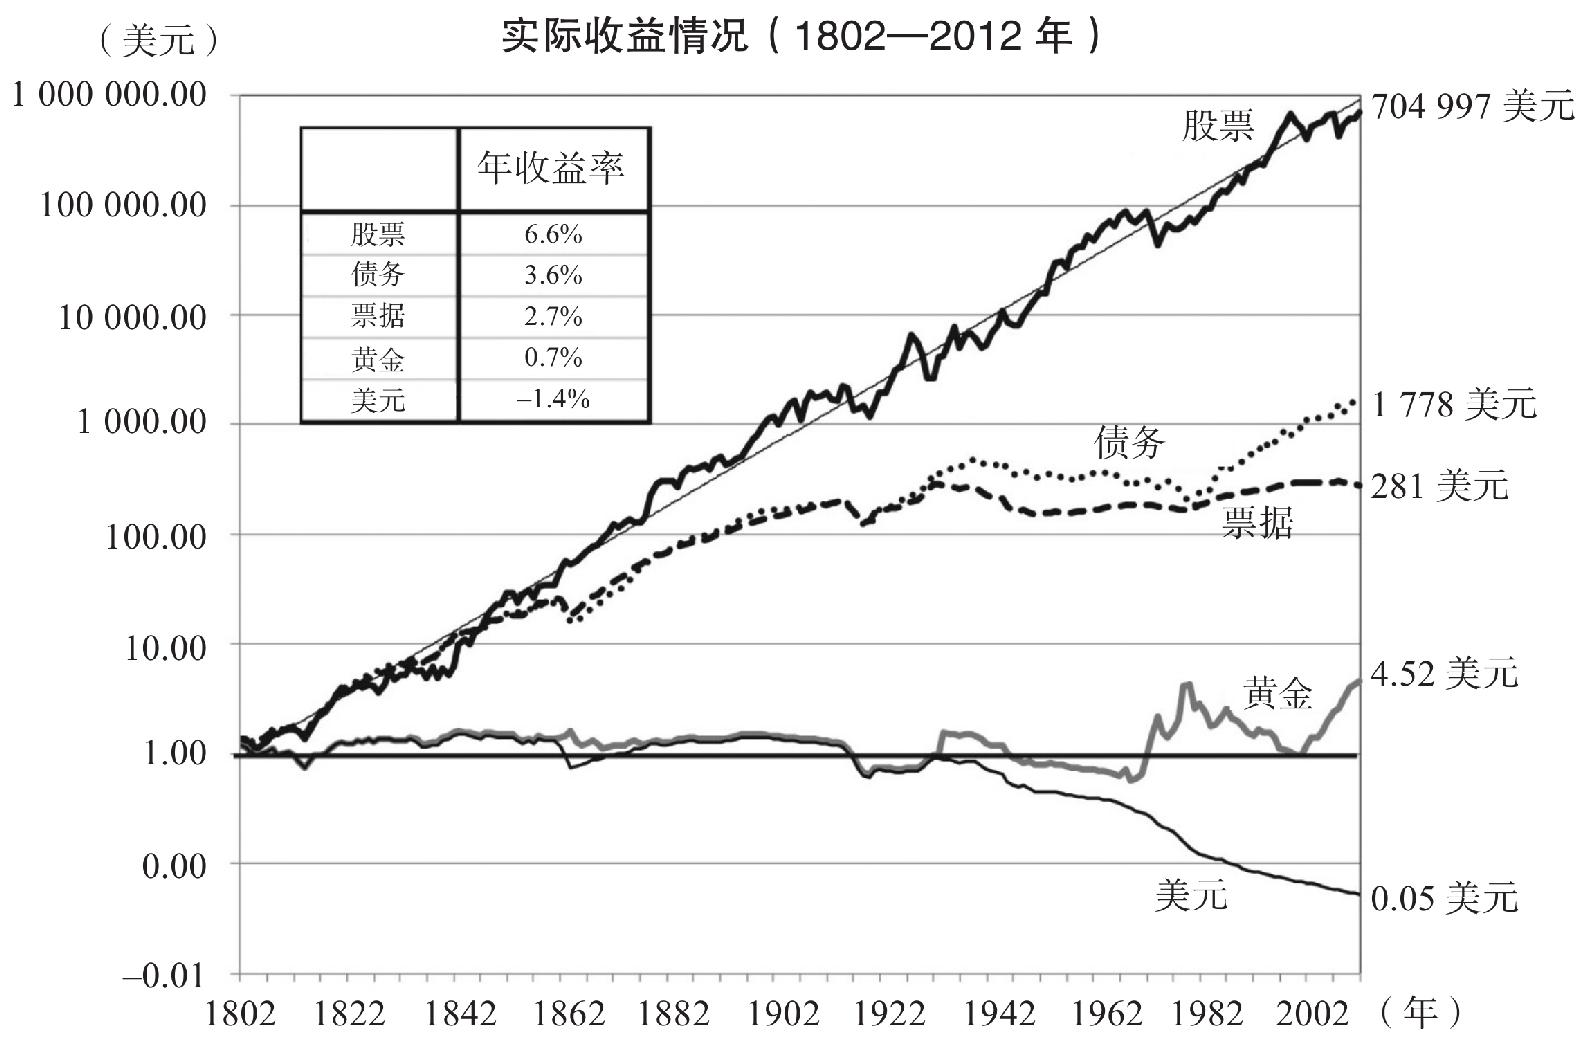
\includegraphics[width=0.96\linewidth,keepaspectratio]{image/23-2.jpg}
\caption{}\label{fig:23-2}
\end{figure}

所以戴维·斯文森把他理想的投资组合设计成了一个赚钱机器，通过极其分散的投资，提供相当稳定的收益，而且因为他进行了长期投资，所以这个投资组合能有充分的时间安然地度过股市的周期性下跌。

我很好奇，想看看这样的资产组合过去的表现怎么样。过去17年中，股票市场波动很大，从1997年4月1日开始，通货膨胀保值国债问世，到2014年3月31日结束。其间，标准普尔500指数的表现就像斗牛表演中一头疯狂的公牛，但是也有下跌的年份，把下跌的年份加在一起计算，市场累计跌幅达到51\%。于是，我组建了一个金融专家团队，测试这个组合的业绩表现，并和同期的指数表现进行对比。你猜猜看，结果怎么样？戴维·斯文森推荐的投资组合完胜股票市场，年化收益率达到7.86\%！在2000—2002年大熊市里，标准普尔500指数下跌接近50\%，斯文森的投资组合相对表现得要稳健多了，在这可怕的几年里，累计亏损只有4.572\%！像其他重仓股票的投资组合一样，斯文森的投资组合在2008年股市大崩盘里也遭受了打击，但是它的表现仍超越标准普尔500指数（下跌31\%，而不是下跌37\%），之后就快速反弹了。\footnote{\label{fn:pdf-23-1}请参考本章末尾各个资产类型的具体指数。过去的业绩并不能保证未来的业绩。}

所以，女士们，先生们，能够真正长期持续战胜市场的投资人，100万人里也难找出1个人，绝对是凤毛麟角，戴维·斯文森就是这样一个极其罕见的绝世高手——用这个投资组合，他持续战胜了市场，一不选股，二不选时，完全只靠资产配置的威力！你可以得到戴维·斯文森的最好的投资建议，就在此地，就在此时。哪怕你读完本章，唯一收获的东西就是戴维·斯文森建议的这个投资组合，我想你也肯定会说：这时间花得值。不过，你要明白的最重要的事情是：即使这个组合业绩比整个股市更好，更稳定，这仍然是一个相当激进的投资组合，它需要你具有强大的心理承受能力，因为拿着自己辛辛苦苦攒的血汗钱做投资，看到账面亏损1/3，很少有人能承受得了，大部分人都被吓得两腿发软，内心崩溃，想赶紧把股票卖掉。那么这个投资组合适合你吗？如果你很年轻，也许会有兴趣做这样重仓股票的资产配置，因为你有足够的时间从任何损失中恢复元气。要是你正准备退休，这个组合也许太危险了。

不过，不要担心。我在后面的内容里会介绍给你几个其他投资大师推荐的投资组合模板，包括瑞·达利欧告诉我的一个很详细的资产配置方案，它好到让我吃惊得要从椅子上摔下来！这个投资组合简直太棒了，所以我要用整整一章来讲。这里先做个提示：瑞·达利欧建议的这个投资组合，其激进程度大大弱于斯文森的投资组合，用同样的时间框架来对它进行回测，瑞·达利欧的投资组合年化收益率更高，而且波动性明显更小——业绩表现要平稳多了，它会给你带来相当高的成长性，而且风险性是最低的，至少在我见过的组合中确实如此。

\begin{BookQuote}
在任何一个做出决定的时刻，你能做的最好的事情就是做正确的事情，第二好的事情是做错误的事情，而你能做得最糟糕的事情，就是什么事情也不做。

\hfill ——西奥多·罗斯福
\end{BookQuote}

但是，我们暂时还要回过头来看一看大局，你如何决定自己的大类资产配置比例：你把自己资产的多大比例用来承受风险、追求成长，你又把多大比例的资产用来获取低收益、追求安全？在你做出选择之前，你必须考虑以下三个因素：

\begin{itemize}
\item 你的生命阶段
\item 你的风险承受能力
\item 你能得到的流动性
\end{itemize}

第一，你的人生还有多少时间让你创造财富，允许你在投资的道路上犯下投资错误，等你年纪大了，生活的主要目的不是赚钱而是花钱了，时间不再允许你犯下投资大错，因为你输不起了。如果你很年轻，当然可以更加激进，因为你有更长的时间来赚钱弥补你的损失。（不过可没有人愿意养成亏损的习惯。）

你的资产配置比例还取决于你的收入水平。如果你能赚很多钱，你就能承担得起犯更多错误的损失，而且还能够有本钱继续投资来弥补这些错误，对不对？

\subsection{真人秀游戏：你愿意冒多大风险？}

谈到风险，什么样的风险是你可以承受的？每个人的看法有很大的不同。我们有些人极度渴望安全。还记得我们前面讲的那六大人类基本需要吗？确定性是排名第一的人类基本需要。但是也有些人渴望不确定性和变化，爱过那种惊险刺激的生活。你必须知道你的个性，然后才能开始动手大干一场。所以，让我们假设你现在正在参加一场真人秀游戏，下面哪些东西是你想要得到的？

\begin{itemize}
\item 1000美元的现金
\item 有50\%的可能赢得5000美元
\item 有25\%的可能赢得10000美元
\item 有5\%的可能赢得100000美元
\end{itemize}

这里还有另外一个游戏：你刚刚攒够了钱，要来一次度假。在你计划休假的3个星期之前，你丢了工作。你会：

\begin{itemize}
\item 取消度假
\item 换个价钱便宜得多的度假计划
\item 继续按计划度假，因为你需要时间做好准备
\item 延长你的假期，因为这也许是你最后一次坐头等舱的机会了
\end{itemize}

罗格斯大学开发了一套在线测试，共20道题，只需要你花5分钟，就能帮助你确定自己属于什么样的风险承受级别。但是真正的答案是什么，你自己心里最清楚。

过去30年，我一直在举办财富大师训练营，参加者来自全球100多个国家，各种各样的人都有，他们通过参加这个完全浸入式的为期4天的财富大师训练课程，改变了他们的财务人生。在这个训练营上，我喜欢跟他们玩一个小游戏，叫作“金钱传递”。我在讲台上告诉听众和其他人“交换金钱”。我说的就是这4个字。通常大家听我这么一说，就会有几分钟的沉默，然后他们充满困惑地开始交换金钱。有些人拿出1美元，有些人拿出20美元，有些人拿出100美元。你可以想象会发生什么情况。人们四处走动，他们互相观察，他们决定如何交换。有些人在协商；有些人把他们的钱全都拿出来了；有些人拿了别人100美元，却只给对方1美元，你可以想象那个人脸上的表情是多么震惊。这种交易持续进行三四分钟之后，我会说：“好了，请坐。”然后我转到下一个话题接着讲。

每次都一样，肯定会有人大叫：“嘿，我想拿回我那100美元！”

我会说：“谁说那是你的100美元？”他说：“拜托，我们只是在玩游戏。”我说：“是的，你怎么知道这个游戏结束了？”通常这个人听到后会满脸困惑，只好坐下来，心里还是非常气愤，毕竟自己失去了100美元。最终他们都从这个游戏中得到了启发：对自己的风险承受力，他们感觉到的和现实完全是两回事。那个家伙觉得自己有很高的风险承受力，但是他才失去了100美元，就让自己愤怒得受不了了。看到这种事，往往让我很震惊。想象一下，要是你亏损了1万美元、10万美元，甚至50万美元，你会有什么样的反应？激进的投资者在相对较短的时期内可能会亏掉这么多钱。人们并不知道他们真正的风险承受力是多大，直到他们发生了相当大的亏损，真实体验到巨大的亏损，他们才会知道自己的实际风险承受能力是多大。

我承受过上帝也会震惊的亏损——在我人生的某阶段我亏掉了几百万美元，可我其实没有那么多钱，结果是我亏的钱比我所拥有的全部资产还要多，这些考验你勇气的事情会惊醒你！但是亏损的数字是大还是小并不重要，亏损100美元或者1000美元就可能让你痛苦得受不了了。输的痛苦远远超过赢的快乐，这正是为什么你的投资弹药库里，一定要有一些像全天候投资组合这样的武器装备，因为只是依靠资产配置，你就可能明显地减少承受重大亏损的风险。

科学研究表明，我们天生痛恨亏损。科学研究还表明，人类并不擅长评估自己获胜的潜在可能性。有时你做了几笔成功的投资，你就开始想：“看来我很擅长做投资。我这个人做什么都行！”因为人类的天性，你才会觉得你能战胜系统。这正是心理学家所说的激励误区，我们大多数人会觉得自己在预测模式上表现得很好，自己会很幸运地中大奖，但其实我们并没有那么好，也没有那么幸运。但当我们有机会中头奖时，我们就会这样想。除此之外，还有什么原因能够解释这么多人热衷于买彩票？斯德哥尔摩大学1981年做的一项研究非常有名。该研究发现，93\%的美国汽车司机觉得他们的开车技术高于平均水平。这种现象甚至还有个专门的名称，叫作乌比冈湖效应。这个名词来源于加里森·基勒书中描写的那个神秘小镇，那里“所有的孩子都高于平均水平”。哎，谁不是觉得自己高于平均水平？但是，在钱的事上，要是你有这样的心理误区，觉得自己比其他所有人都要好，那会让你付出惨重的代价。

要是你是个男人，你会觉得很内疚，自己竟然有这种生物化学上的偏见。男性睾酮会让人过度自信。一个又一个研究表明，女人往往能成为更好的投资者，因为她们并不会高估自己准确预测未来的能力。有的时候，自信是好事，但也有很多时候，自信是坏事，会起反作用。你只要看一看小孩子就明白了。“我是超人！我要飞喽！你看我敢跳下屋顶！”我完全可以说，如果你是位女性读者，你做投资天生就比男性有优势。

当市场上涨再上涨的时候，投资者就会陶醉在盈利之中，我赚钱了，我又赚钱了。每个人内心都会受到诱惑。正是这种心理让投资者出了大问题。这样过度自信的结果是，他们把自己大部分的钱，甚至所有的钱，都投到股票等热门投资上，而这些投资应该属于风险/成长水桶中的资产——不只是70\%，有时是80\%、90\%，甚至是100\%。股市和楼市很火的时候，有些人甚至借钱来投资股票和房子，因为他们相信这些股票永远会上涨，直到亲眼看到股市不再上涨，下跌了，又下跌了，他们才不相信股市会永远上涨。因为他们的资产配置做得很糟糕，把大部分钱都投在股票或房产这样的野马身上，后来他们把钱全部亏光了，有的人甚至还欠了一屁股债。这些人失败的原因是，等到他们听说股票市场（或者是黄金，或者是房地产，或者是商品期货，或者是其他资产）是个赚钱的好地方时，这个市场的泡沫通常就快要破掉了。你需要事先妥善地安排和设置好一个系统，以确保你不会受到引诱，不会把太多的钱投在任何单一的市场上或者单一的资产类型上，不会把太多的钱放到你的风险/成长水桶里。

所有这些东西听起来非常简单，像是常识，特别是那些资深投资者会觉得自己什么都知道，什么都明白。但是有时候越是水平高的投资者，因为他们太想追求成功了，结果越容易偏离轨道掉到山沟里。他们忘记了那些投资常识。

当然，总有些投资者根本不听这些道理，他们做投资一点儿不讲道理，不讲理性，“非理性繁荣”就是这些人给煽起来的。他们相信了那个最大的投资谎言：“这次肯定不一样。”我知道有好几十件这样的真人真事，故事的结局都很悲惨。就拿乔纳森来说吧（为了保护他的隐私，我就不讲他的真名了），我这个朋友做生意发了笔财，后来他把所有东西都卖掉，拿到一笔钱，去投资当时很火的拉斯维加斯房地产市场。一开始他赚了些钱，于是他加倍投资，疯狂地借钱来持续开发房地产项目。每一次，乔纳森来参加我办的投资理财大师训练营，他都会听到我一再重复讲资产配置非常重要，要学会“落袋为安”，把你的一些盈利放进你的安全/安心水桶里，不要把你所有的鸡蛋放在同一个篮子里，不管现在这个篮子看起来多么诱人。乔纳森很信任我这个人，也很信任我的投资理财大师训练营，正是参加这个训练营，他才让企业盈利超过10倍的，不然他哪里有钱来做房地产投资？他卖掉了自己的公司，拿到了1.5亿美元。我给他的建议是，现在是时候把赢的钱拿出来放进安全/安心水桶里了，但是他没有听我的。现在他才知道自己太自以为是了，把我的话都当成了耳旁风。他想成为亿万富翁，他觉得自己做得很对，正在大步奔向目标。但是后来你也知道，拉斯维加斯发生了房地产大崩盘。你猜猜房价暴跌了多少？2007—2012年暴跌了61\%。乔纳森所有的财产都亏光了，这还不止，两手空空的他还有5亿美元的债务要还。

\begin{figure}[htbp]
\centering
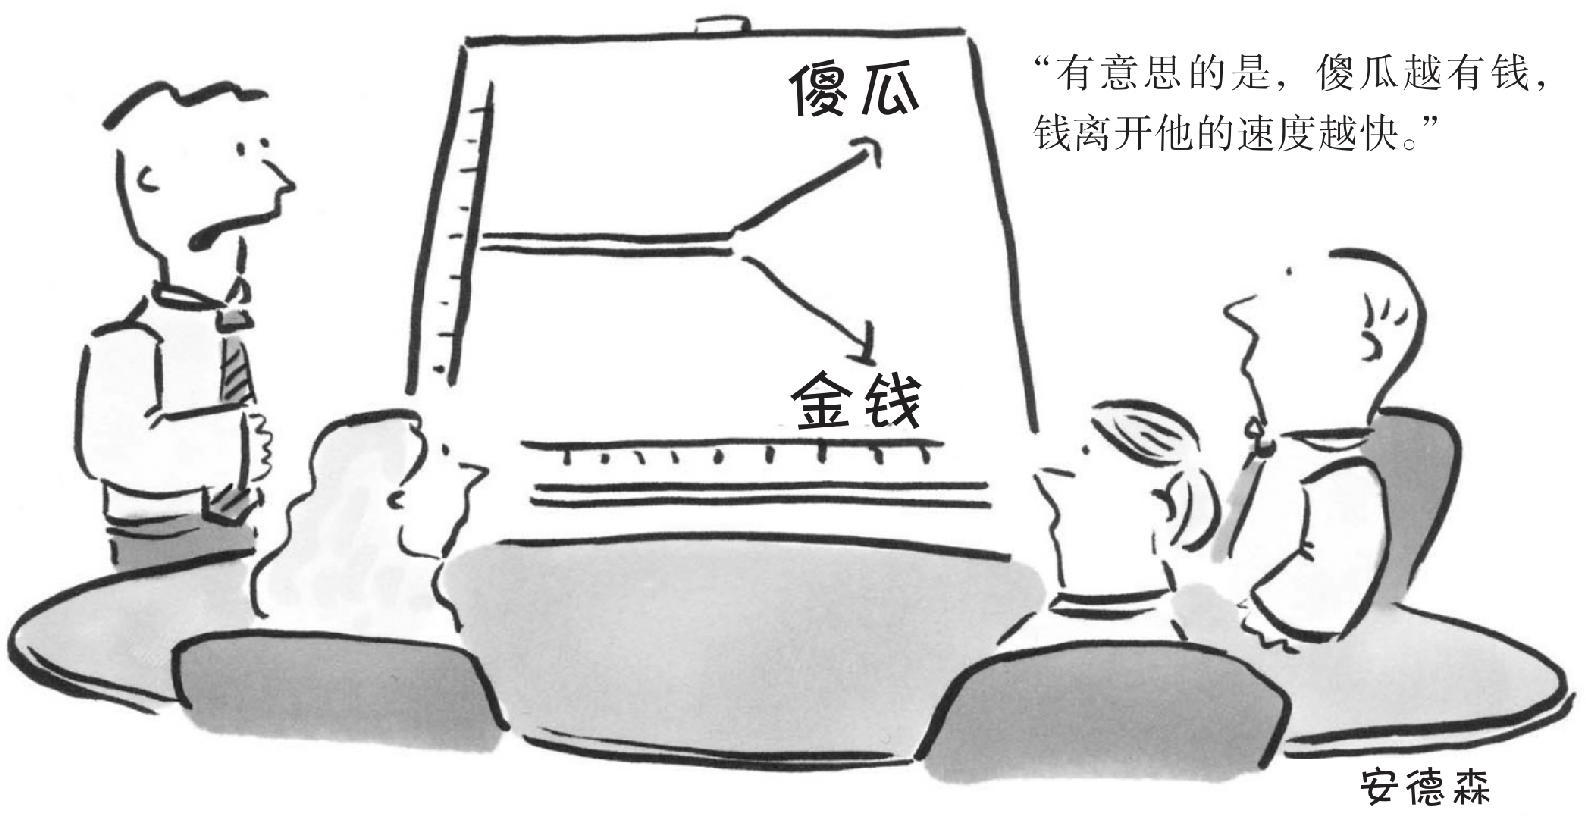
\includegraphics[width=0.80\linewidth,keepaspectratio]{image/23-3.jpg}
\caption{}\label{fig:23-3}
\end{figure}

我真诚地希望，所有这样的投资蠢事从此再也不会发生。如果说这一章你有什么东西应该牢记在心的，那就是把你所有的钱都放在风险/成长水桶里，你就是自找死路。这正是为什么很多专家估计，从任何一个10年来看，几乎95\%的投资者都是亏钱的。一般来说，他们总是在市场大涨浪潮涌起之后追涨买入（包括房地产、股票、黄金），而在市场下跌的时候，他们就像岩石一样坠落。暴涨之后必有暴跌，他们必定会受到巨大财务损失的打击。

我们的投资建议再好，有些人就是不听。他们必须用最痛苦的方式来学习，吃尽苦头，才能吸取经验教训。但是为了避免这类痛苦的教训，帮助你决定什么样的选择对你才是正确的，我需要提醒你，找一个没有利益冲突的、独立的受托人投资顾问，这才是一个正确的选择。请注意那些职业运动员，那些在他们从事的体育项目上成绩属于顶尖水平的男运动员或者女运动员，他们总会找个教练，帮助他们保持顶尖的成绩。为什么他们要这样做？因为教练会注意到，什么时候他们在比赛时偏离正轨了，然后帮助他们做些小的调整，结果会产生巨大的效果。同样的事情也适用于你的投资理财。一个非常棒的受托人财务顾问就像一个好教练，他会帮助你保持一直在正道上前进。当你开始像个青少年一样冲动，追逐业绩，在市场上涨中过于陶醉，迷失自我时，或者在市场下跌中过于恐惧，想要逃离时，他们会及时相劝，他们可以说服你离开悬崖，避免你做出一个致命的错误投资决策。

\subsection{选个数字，随便一个数字}

现在是时候估算一下你的两个水桶的资产配置比例了！比如，你现在拿到手10000美元的奖金（或者你已经积累了10万美元、20万美元、50万美元、100万美元，甚至更多的钱），你决定把这些钱都拿去投资。到现在为止，你读了这么多，学了这么多，知道了这么多，这些钱你该如何把它们分散进行投资？你的新投资哲学是什么？你的钱有多大比例会被放在安全/安心水桶里，在安全的环境下保持稳定增长？还有多大比例的钱你愿意放到风险/成长水桶里，去冒险追求更高的潜在增长？

你可能听说过那个古老的经验法则（约翰·博格称之为粗略估计方法）：你的年龄有多大，投资债券的比例就有多大。换句话说，用100减去你的年龄，就是你可以投资到股票上的资产比例。如果你现在40岁了，那么你应该把60\%（100\%－40\%）的资金投资在股票上，这属于你的风险/成长水桶，40\%的资金投资在债券上，这属于你的安全/安心水桶。等你到了60岁，你投资股票的比例应该是40\%（100\%－60\%），而投资债券的比例应该是60\%。但是，这样的资产配置比例已经远远不符合当代的现实情况了。股票和债券二者的波动性都大大增加了，而且现在的人活得比过去长多了。

那么什么样的资产配置比例才适合你？你希望更加激进，冒更多的风险，就像戴维·斯文森建议的重仓股票的投资组合一样，30\%的资金投资债券，追求安全，而70\%的资金投资股票，承受风险吗？这意味着你那10000美元的资金，要拿出30\%，也就是3000美元，放进安全/安心水桶中，而70\%的资金，也就是7000美元，放进你的风险/成长水桶里。（如果你有100万美元，这个资产配置比例不变，你就要把30万美元放进安全/安心水桶里，70万美元放进风险/成长水桶里。）你真的承受得起这样三七分的资产配置吗？你是不是有足够的现金？你是不是有足够的时间？你是不是足够年轻？你是不是需要更加保守一点，像很多养老金机构那样，来个六四分或者五五分？还是你年纪大了，接近退休了，那么你希望是二八分？重要的不是大多数人是怎么做的，重要的是你自己会怎么做。这样做既符合你的财务需要，又符合你的感情需要。

我知道，这是一个相当个人化的选择，即使是最聪明的投资理财明星，有的时候也得想很长时间，而且要花很多工夫思考，到底什么样的资产配置比例更适合自己和自己的家庭。我和摩根大通资产管理公司的玛丽·卡拉汉·厄道斯交谈的时候，我问她：“构建资产组合的时候，你用的是什么标准？如果你必须给你的孩子构建一个资产配置，那么这个配置会是什么样的？”

“我有三个女儿。”她告诉我，“当然，她们三个年纪不一样大。她们三个人的能力也各有不同，以后随着时间推移，她们的能力也会变化，我不知道她们长大之后会变成什么样子。一个可能花钱比其他人更多一些；一个也许希望找个好的工作环境，能挣更多的钱；一个也许会更加喜欢做慈善。三个人都有可能遇上什么事情，比如健康出了问题。一个会结婚，一个也许不会结婚；一个会要小孩，一个可能不要孩子。不同的偏好，不同的事，不同的时间，在每个人身上会有不同的排列组合，还会随着时间发生变化。因此，尽管从出生第一天起，我就给她们设计了一个资产配置，但是这个资产配置还必须随着时间的变化而变化。”

“资产配置比例的变化要基于人们的风险偏好的变化而变化，因为随着时间推移，你不可能一直让这个人保持一个完美的资产配置，只有适合他的资产配置对于他来说才是完美的。如果处于人生的最后阶段，有个人可能过来和我说：‘我只想要国债，让我能够晚上安安心心地睡觉，一点儿也不用担心。’对于他来说，这也许是最好的办法。”

我和她说：“因为这符合他的情感需要，对不对？最终，生活不仅是钱的事情。”

“太对了，托尼。”她说，“如果我把投资组合的一半资金拿出来放到股市上，可能会多赚些钱，但是股市经常大涨大跌，会让人们承受很大的心理压力，破坏人们生活中的幸福感。我何必要这样做？”

“投资的目的是什么？”我问，“难道不是为了确定我们为自己也为家人创造了经济上的自由吗？”

“你说的对，投资其实就是为了能获得经济自由，能做你想做的事。”她说，“但是你不值得为此付出高昂的代价，压力，紧张，不舒服，特别是在股市表现非常糟糕的时候，你的情绪也会非常糟糕。”

玛丽·卡拉汉·厄道斯绝对是世界上极优秀的投资理财专家之一，从她给三个女儿做资产配置的经验中，你能学到的经验是什么？积累你的财富更加重要的是，做投资理财这件事，要用一种适合自己的方式，必须能给自己带来心灵的平静。赚钱了，心却乱了，生活也乱了，那就不值了。

那么你的安全/安心水桶和风险/成长水桶间的大类资产配置比例应该是多少？写下来你理想的资产配置比例，让这些数字从脑子里的想象，变成真实的白纸黑字！这些配置比例数字让你感觉舒服吗？绕着这些数字走两圈。想象你按照这些数字比例做了资产配置，这个数字成了你生活的一部分。持有按照这个数字比例做的资产配置！因为按照这个数字比例所做的资产配置比例，是让你得到心灵平静的关键所在，也是决定你财务未来的关键所在。

写好了吗？

好了。你刚刚做出了人生最重要的投资决策。一旦你知道你的资产配置比例是什么，你就不要再改变了，除非你进入了人生新的阶段，或者你的个人情况出现了巨大变化。一般情况下，你要一直坚持这样的资产配置比例，让投资组合保持平衡。我会展示给你如何做到再平衡，就在这部分后面的内容里。

你是不是还很在意如何做出正确的选择？只要记住一点，你找个受托人投资顾问来帮助你，这就够了。你并不需要有很多财富，才能请得起投资顾问——你一分钱没有也没有关系，你可以利用互联网上的相关服务。

顺便说一下，我还没有给你讲完呢！在这两个水桶之内进行资产配置，还有一些方法可以增加你的投资收益，我们很快就会讲这些方法。

现在你已经明白了这些原则，而且已经做出了决定，多大比例的钱放进风险/成长水桶，多大比例的钱放进安全/安心水桶。让我告诉你最好的消息：我访问了50位世界上最成功的投资大师，最聪明的理财大师，我从他们那里找到了一些方法，让你可以鱼与熊掌兼得，既能得到风险/成长水桶那样的高收益，又能得到安全/安心水桶那样的低风险。这个最重要的投资理财建议就是：“千万不要亏本！”每个投资者都非常赞同。但是对于很多投资者来说，这意味着你要满足于只在安全/安心水桶里得到的平庸收益率。后面几章，我会和你分享一个好的投资方法：如何既能拥有上行的潜在收益，又没有下行的风险；如何能够得到相当大的增长，同时又没有相当大的风险。我知道这听起来很荒唐很离谱，但是这是真实的，会让人非常兴奋。

你能学完这一章不容易，你一定下了很大功夫，付出了很多努力。我非常高兴地告诉你，下一章就容易多了，而且纯粹都是讲开心快乐的事情。现在我将要打开第三个水桶，到现在我们还没有谈论，但是你肯定会非常喜欢第三个水桶的，因为这个水桶里充满了乐趣，充满了灵感和启发，可以给你带来更高品质的生活，而不是让你再过几十年才能享受得到。现在，让我们去发现哪些资产可以进入你的梦想水桶吧。

\subsection{各个资产类型的具体指数}

戴维·斯文森提供了每个资产类型的具体配置比例，但是他并没有提供代表各个资产类型的具体指数。独立的分析师会运用下面的指数代表每个资产类型，并假设是这个投资组合让每个季度进行再平衡的。请注意，过去的业绩并不能保证未来的业绩。相反，我提供给你的历史业绩数据，在这里是为了讨论和描述基本的原则的。

20\%威尔逊5000全球整体市场指数

20\%英国富时房地产投资信托指数

20\%MSCI国家指数

15\%巴克莱长期信用指数

15\%巴克莱国库债券指数

10\%MSCI新兴市场国家指数
